% +------------------------------------------------------------------------+
% | CGAL Reference Manual:  generators.tex
% +------------------------------------------------------------------------+
% | Geometric object generators.
% |
% | 09.06.1997   Lutz Kettner
% | 

% +------------------------------------------------------------------------+


\section{Introduction}
A variety of generators for geometric objects are provided in \cgal.
They are useful as synthetic test data sets, e.g.~for testing
algorithms on degenerate object sets and for performance analysis.

Two kinds of point generators are provided: first, random point
generators and second deterministic point generators. Most random
point generators and a few deterministic point generators are provided
as input iterators.  The input iterators model an infinite sequence of
points. The function \ccc{CGAL::copy_n()} can be used to copy a
finite sequence; see Section~\ref{sectionCopyN}. The iterator adaptor
\ccc{Counting_iterator} can be used to create finite iterator
ranges; see Section~\ref{sectionCountingIterator}.
Other generators are provided as functions that write to output
iterators. Further functions add degeneracies or random perturbations.

\ccIndexSubitem[c]{generator}{2D point}
\ccIndexSubitem[c]{point, 2D}{generator}
In 2D, we provide input iterators to generate random points in a disc
(\ccc{Random_points_in_disc_2}), 
in a square (\ccc{Random_points_in_square_2}),
on a circle (\ccc{Random_points_on_circle_2}), 
on a segment (\ccc{Random_points_on_segment}),
and on a square (\ccc{Random_points_on_square_2}).
For generating grid points we provide three functions,
\ccc{points_on_segment_2},
\ccc{points_on_square_grid_2} that write to output iterators and
an input iterator \ccc{Points_on_segment_2}.

\ccIndexSubitem[c]{generator}{3D point}
\ccIndexSubitem[c]{point, 3D}{generator}
For 3D points, input iterators are provided for random points uniformly 
distributed in a sphere (\ccc{Random_points_in_sphere_3})
or cube (\ccc{Random_points_in_cube_3}) or on the boundary of a sphere
(\ccc{Random_points_on_sphere_3}).
For generating 3D grid points, we provide the function 
\ccc{points_on_cube_grid_3} that writes to
an output iterator.

We also provide two functions for generating more complex geometric objects.
The function \ccc{random_convex_set_2} computes a random convex planar
point set of a given size where the points are drawn from a specific
domain and \ccc{random_polygon_2} generates a random simple polygon from
points drawn from a specific domain.  

\subsection{Random Perturbations}
\ccIndexMainItem{random perturbations}

Degenerate input sets like grid points can be randomly perturbed by a
small amount to produce {\em quasi}-degenerate test sets. This
challenges numerical stability of algorithms using inexact arithmetic and
exact predicates to compute the sign of expressions slightly off from zero.
For this the function \ccc{perturb_points_2} is provided.

\subsection{Adding Degeneracies}
\ccModifierCrossRefOff
\ccIndexSubitem{degeneracies}{adding to input}
\ccModifierCrossRefOn

For a given point set certain kinds of degeneracies can be produced
by adding new points. The \ccc{random_selection()} function is
useful for generating multiple copies of identical points.
The function \ccc{random_collinear_points_2()} adds collinearities to
a point set.

\subsection{Support Functions and Classes for Generators}

The function \ccc{random_selection} chooses $n$ items at random from a random
access iterator range which is useful to produce degenerate input data
sets with multiple entries of identical items.

\section{Example Generating Degenerate Point Sets}

We want to generate a test set of 1000 points, where 60\% are chosen
randomly in a small disc, 20\% are from a larger grid, 10\% are duplicates
points, and 10\% collinear points. A random shuffle removes the
construction order from the test set. See \ccTexHtml{%
Figure~\ref{figurePointGenerator}}{Figure <A HREF="#PointGenerators">&#x261E;</A>}
for the example output.

\ccIncludeExampleCode{Generator/random_degenerate_point_set.cpp}

\begin{ccTexOnly}
  \begin{figure}
    \noindent
    \hspace*{0.025\textwidth}%
    \begin{minipage}{0.45\textwidth}%
      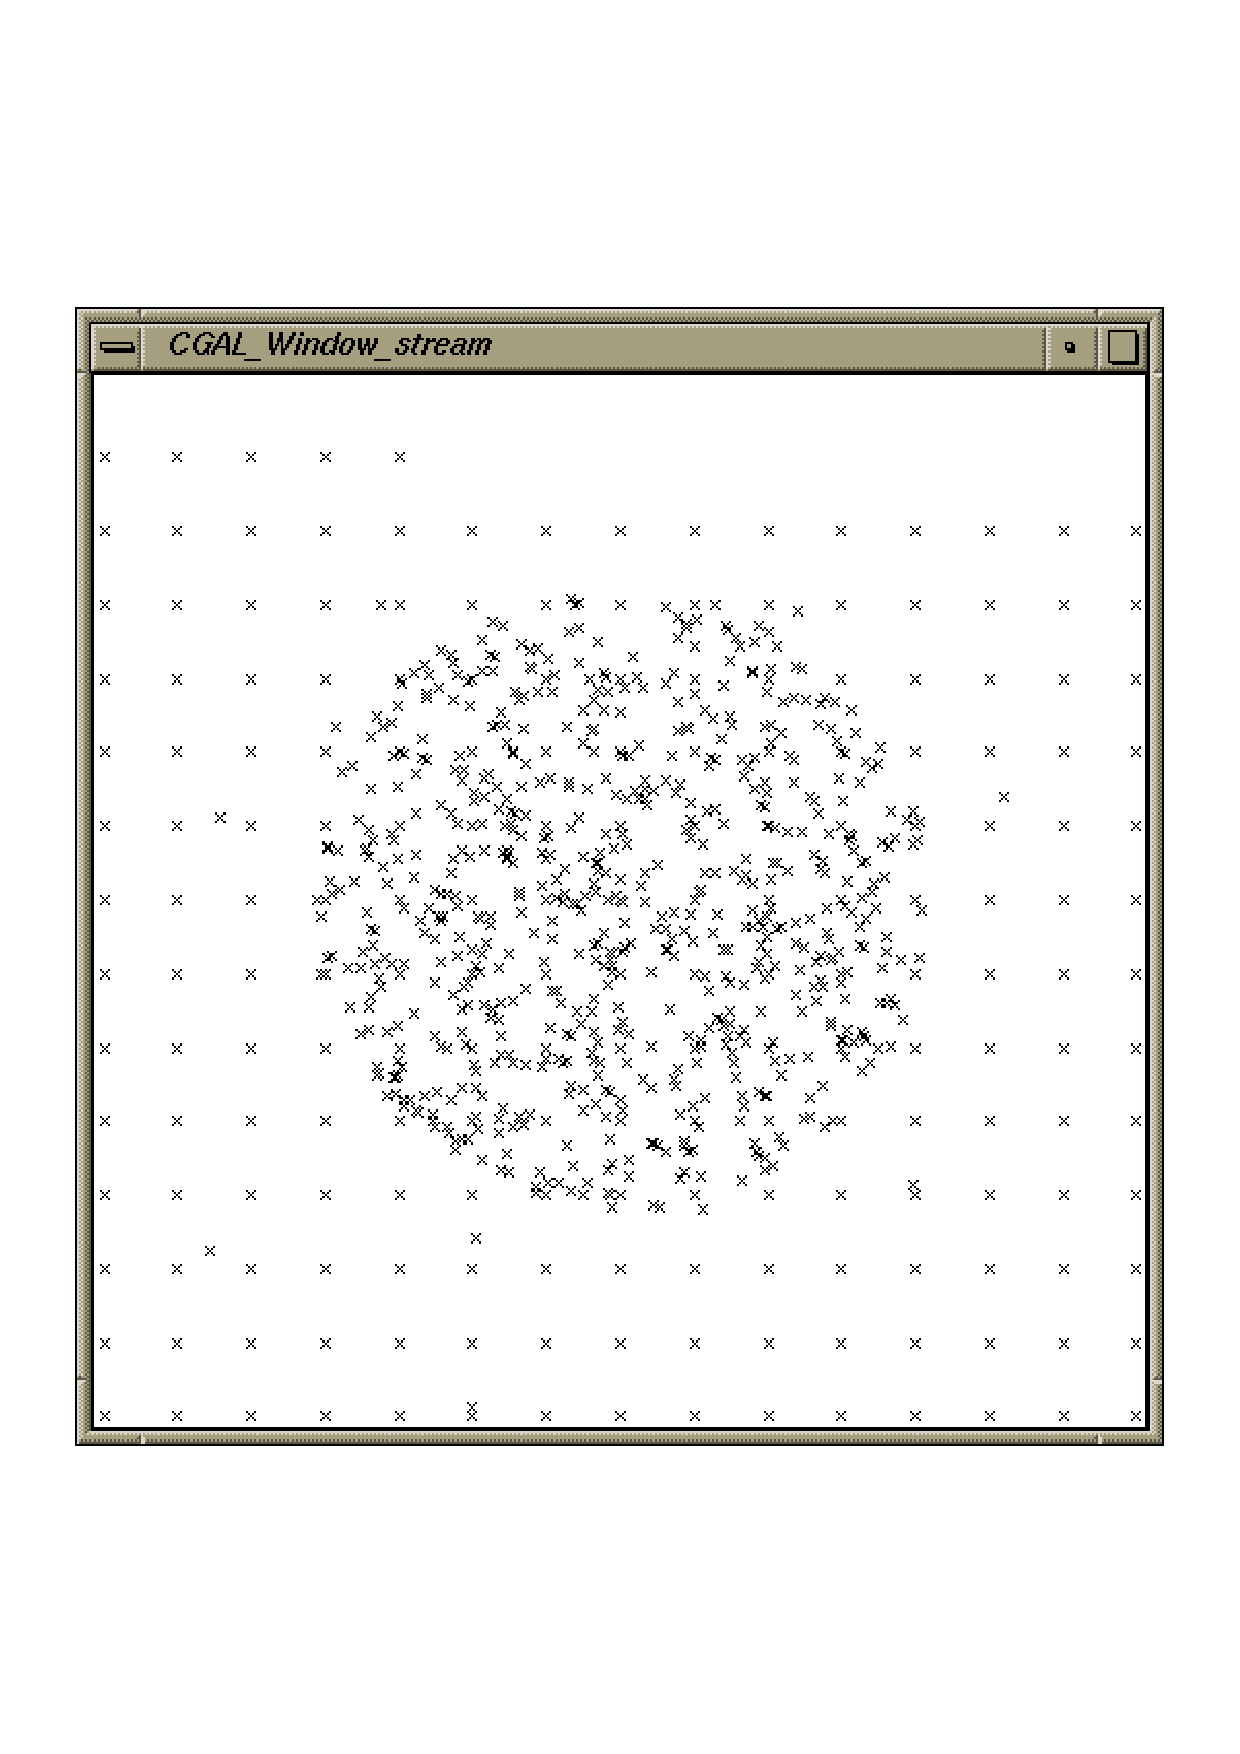
\includegraphics[width=\textwidth]{Generator/generators_prog1}
      \caption{Output of example program for point generators.}
      \label{figurePointGenerator}
    \end{minipage}%
    \hspace*{0.05\textwidth}%
    \begin{minipage}{0.45\textwidth}%
      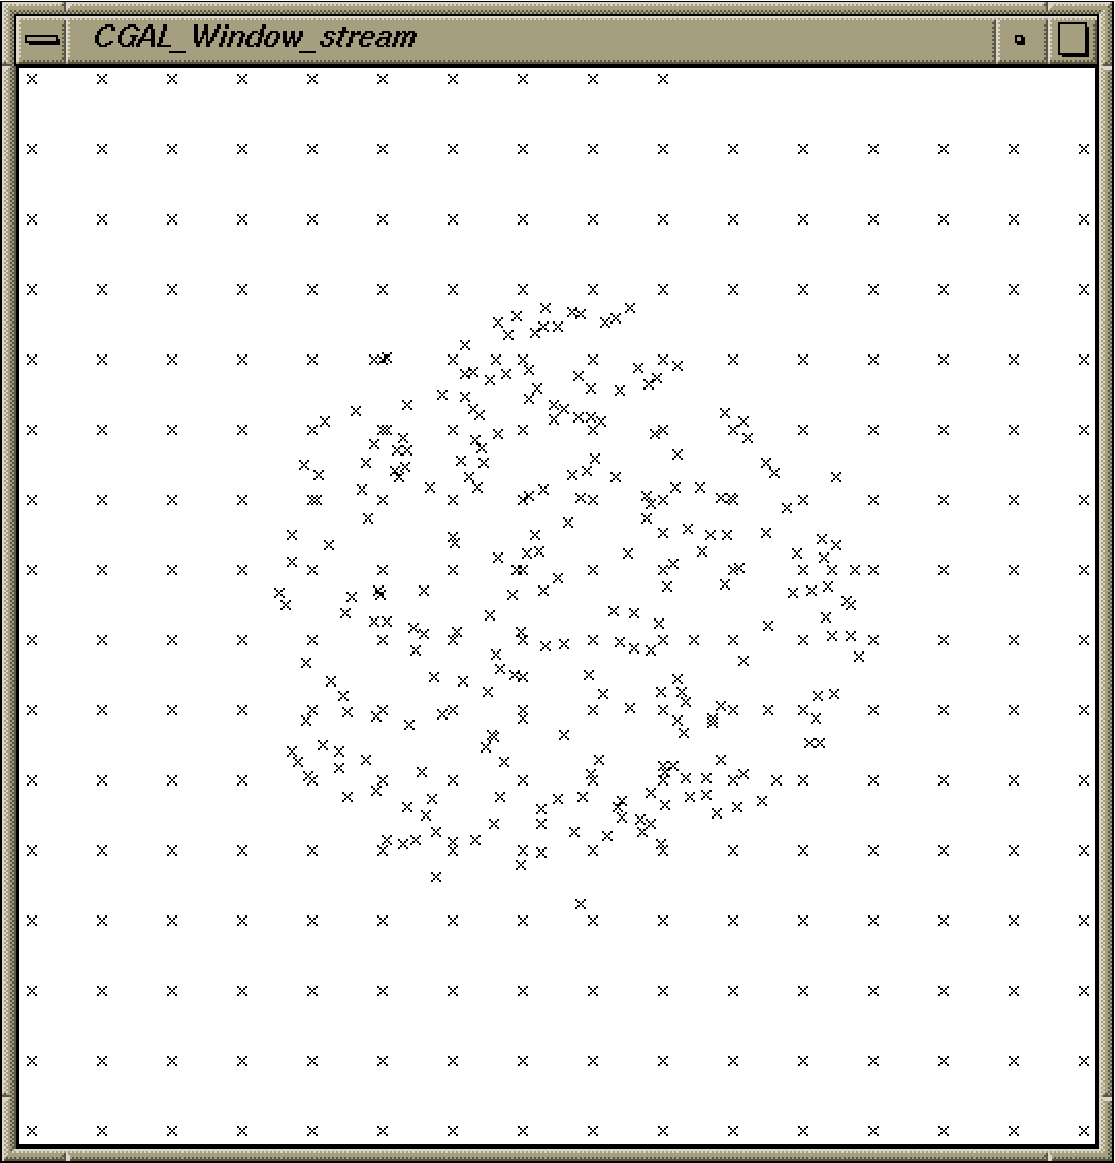
\includegraphics[width=\textwidth]{Generator/generators_prog2}
      \caption{Output of example program for point generators working
        on integer points.}
      \label{figureIntegerPointGenerator}
    \end{minipage}%
  \end{figure}
\end{ccTexOnly}

\begin{ccHtmlOnly}
  <A NAME="PointGenerators">
  <TABLE><TR><TD ALIGN=LEFT VALIGN=TOP WIDTH=60%>
    <A HREF="./generators_prog1.gif">Figure:</A>
    Output of example program for point generators.
  </TD><TD ALIGN=LEFT VALIGN=TOP WIDTH=5% NOWRAP>
  </TD><TD ALIGN=LEFT VALIGN=TOP WIDTH=35% NOWRAP>
    <A HREF="./generators_prog1.gif">
        <img src="./generators_prog1_small.gif" 
             alt="Point Generator Example Output"></A>
  </TD></TR></TABLE>
\end{ccHtmlOnly}

\section{Example Generating Grid Points}

The second example demonstrates the point generators with integer
points. Arithmetic with \ccc{double}s is sufficient to produce
regular integer grids. See \ccTexHtml{%
Figure~\ref{figureIntegerPointGenerator}}{Figure 
  <A HREF="#IntegerPointGenerators">&#x261E;</A>}
for the example output.

\ccIncludeExampleCode{Generator/random_grid.cpp}

\begin{ccHtmlOnly}
  <A NAME="IntegerPointGenerators">
  <TABLE><TR><TD ALIGN=LEFT VALIGN=TOP WIDTH=60%>
    <A HREF="./generators_prog2.gif">Figure:</A>
        Output of example program for point generators working
        on integer points.
  </TD><TD ALIGN=LEFT VALIGN=TOP WIDTH=5% NOWRAP>
  </TD><TD ALIGN=LEFT VALIGN=TOP WIDTH=35% NOWRAP>
    <A HREF="./generators_prog2.gif">
        <img src="./generators_prog2_small.gif" 
             alt="Integer Point Generator Example Output"></A>
  </TD></TR></TABLE>
\end{ccHtmlOnly}%



% +------------------------------------------------------------------------+
%\newpage
\section{Examples Generating Segments\label{sec:segment_example}}
\lcTex{\ccIndexSubitemBegin[c]{generator}{segment}}

The following two examples illustrate the use of the generic functions
from Section~\ref{sectionGenericFunctions} like
\ccc{Join_input_iterator_2}%
\lcTex{\ccIndexGlobalFunction{Join_input_iterator_2}} to generate 
composed objects from other
generators -- here two-dimensional segments from two point generators.

We want to generate a test set of 200 segments, where one endpoint is
chosen randomly from a horizontal segment of length 200, and the other
endpoint is chosen randomly from a circle of radius 250. See
\ccTexHtml{Figure~\ref{figureSegmentGenerator}}{Figure <A
  HREF="#SegmentGenerator">&#x261E;</A>} for the example
output.

\begin{ccTexOnly}
  \begin{figure}
    \noindent
    \hspace*{0.025\textwidth}%
    \begin{minipage}[t]{0.45\textwidth}%
      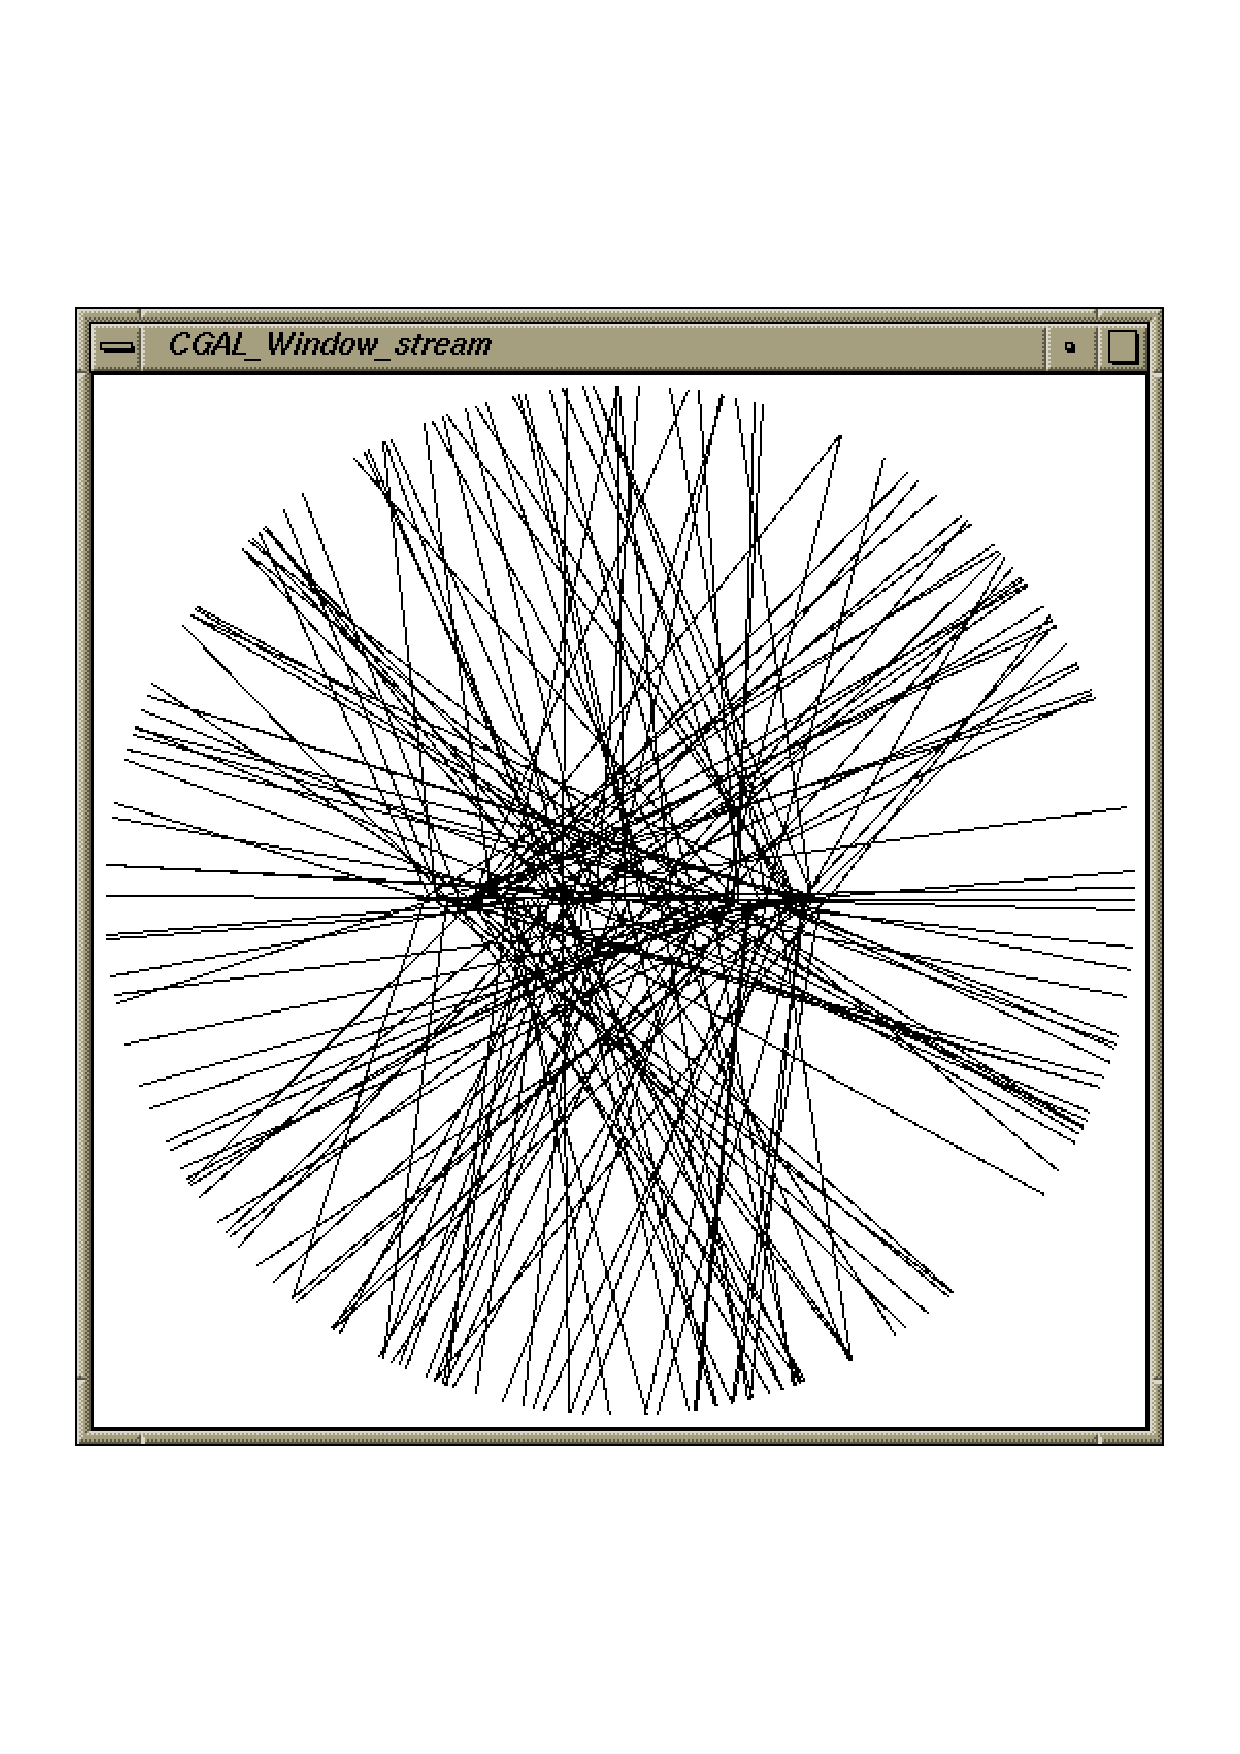
\includegraphics[width=\textwidth]{Generator/Segment_generator_prog1}
      \caption{Output of the first example program for the generic generator.}
      \label{figureSegmentGenerator}
    \end{minipage}%
    \hspace*{0.05\textwidth}%
    \begin{minipage}[t]{0.45\textwidth}%
      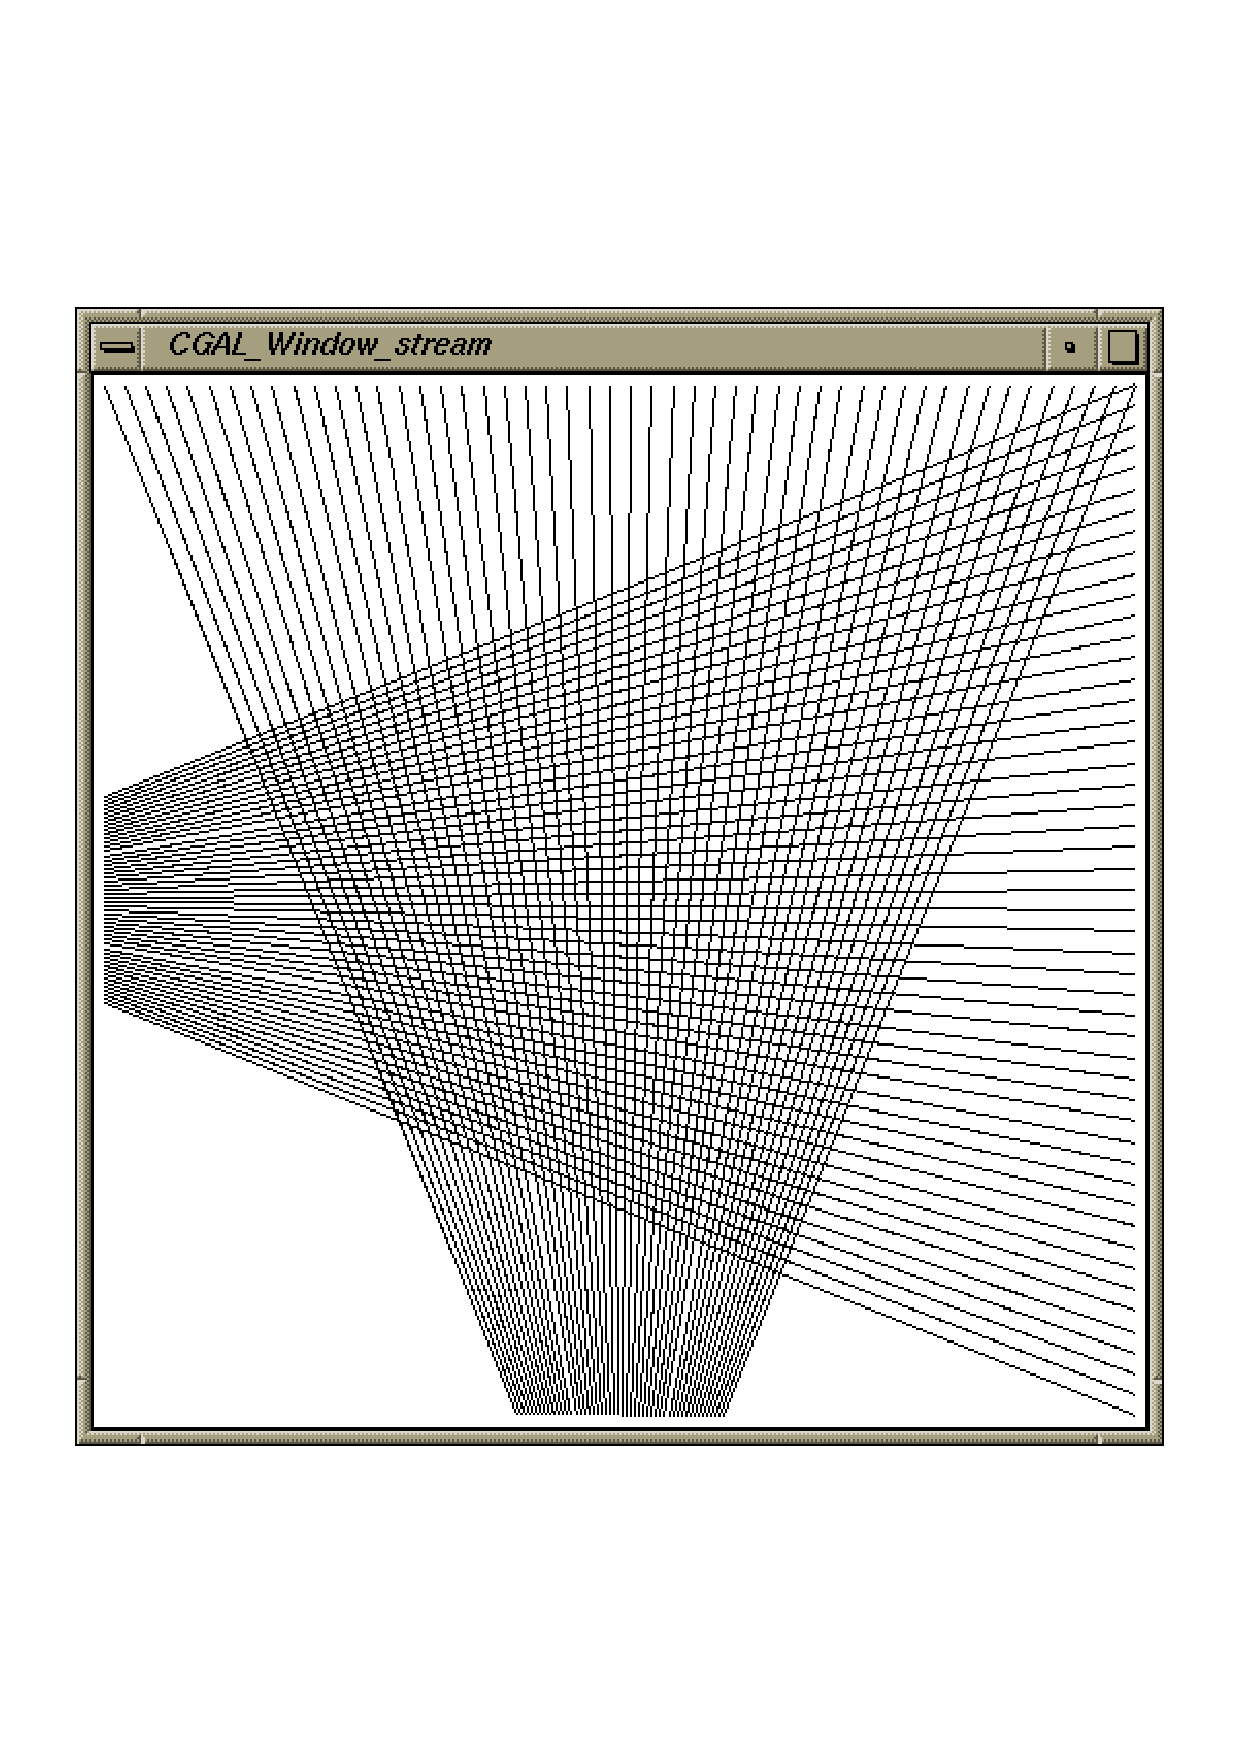
\includegraphics[width=\textwidth]{Generator/Segment_generator_prog2}
      \caption{Output of the second example program for the generic
        generator without using intermediate storage.}
      \label{figureSegmentGeneratorFan}
    \end{minipage}%
  \end{figure}
\end{ccTexOnly}

\ccIncludeExampleCode{Generator/random_segments1.cpp}

\begin{ccHtmlOnly}
  <A NAME="SegmentGenerator">
  <TABLE><TR><TD ALIGN=LEFT VALIGN=TOP WIDTH=60%>
    <A HREF="./Segment_generator_prog1.gif">Figure:</A>
    Output of example program for the generic segment generator.
  </TD><TD ALIGN=LEFT VALIGN=TOP WIDTH=5% NOWRAP>
  </TD><TD ALIGN=LEFT VALIGN=TOP WIDTH=35% NOWRAP>
    <A HREF="./Segment_generator_prog1.gif">
        <img src="./Segment_generator_prog1_small.gif" 
             alt="Segment Generator Example Output"></A>
  </TD></TR></TABLE>
\end{ccHtmlOnly}

The second example generates a regular structure of 100 segments; see 
\ccTexHtml{Figure~\ref{figureSegmentGeneratorFan}}{Figure <A
  HREF="#SegmentGeneratorFan">&#x261E;</A>} for the example
output. It uses the \ccc{Points_on_segment_2}%
\lcTex{\ccIndexGlobalFunction{Points_on_segment_2}} iterator,
\ccc{Join_input_iterator_2}%
\lcTex{\ccIndexGlobalFunction{Join_input_iterator_2}}
and \ccc{Counting_iterator} %\lcTex{\ccIndexGlobalFunction{Counting_iterator}}
to avoid any intermediate storage of the generated objects until they are
used, which in this example means copied to a window stream.

\ccIncludeExampleCode{Generator/random_segments2.cpp}

\begin{ccHtmlOnly}
  <A NAME="SegmentGeneratorFan">
  <TABLE><TR><TD ALIGN=LEFT VALIGN=TOP WIDTH=60%>
    <A HREF="./Segment_generator_prog2.gif">Figure:</A>
    Output of example program for the generic segment generator using
    pre-computed point locations.
  </TD><TD ALIGN=LEFT VALIGN=TOP WIDTH=5% NOWRAP>
  </TD><TD ALIGN=LEFT VALIGN=TOP WIDTH=35% NOWRAP>
    <A HREF="./Segment_generator_prog2.gif">
        <img src="./Segment_generator_prog2_small.gif" 
             alt="Segment Generator Example Output 2"></A>
  </TD></TR></TABLE>
\end{ccHtmlOnly}
\lcTex{\ccIndexSubitemEnd[c]{generator}{segment}}


% +--------------------------------------------------------+
% restore default column and paragraph layout
\ccParDims
\cgalColumnLayout



% +--------------------------------------------------------+
% restore default column and paragraph layout
\ccParDims
\beforecprogskip\parskip
\aftercprogskip0pt


% EOF
